\documentclass[preview]{standalone}

\usepackage{amssymb}
\usepackage{physics}
\usepackage{tikz}
\usetikzlibrary{positioning}
\usetikzlibrary{arrows}

\newcommand{\R}{\mathbb{R}}
\newcommand{\D}{\mathrm{D}}


\begin{document}

\begin{figure}[h]
\centering
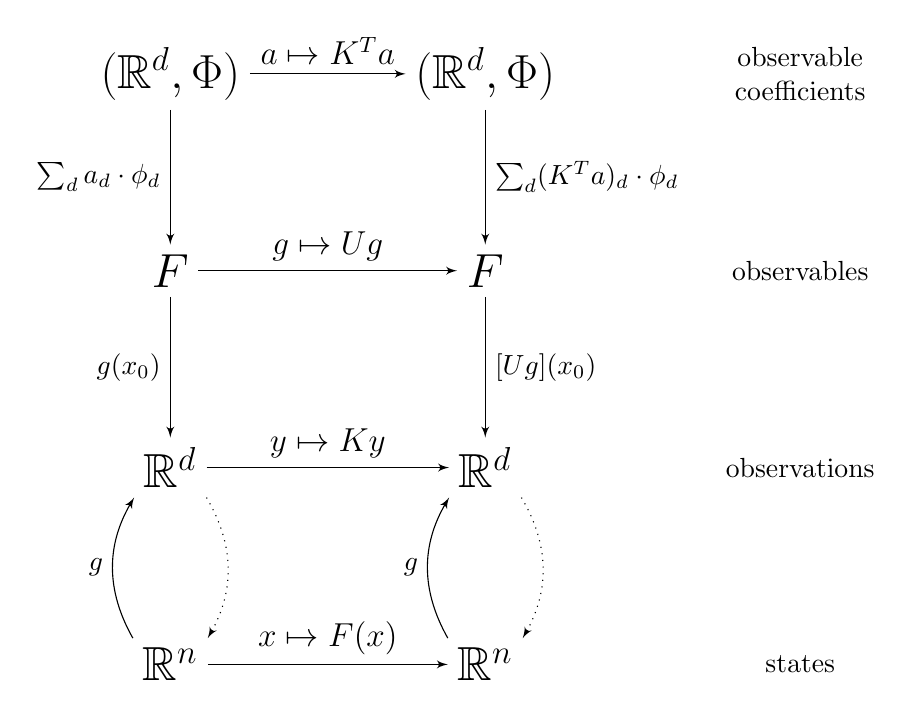
\begin{tikzpicture}[fill=gray]

\tikzset{
    vertex/.style={circle,draw,minimum size=1.5em},
    edge/.style={->,> = latex'}
}
% variables
\def\ylen{2.5}
\def\xlen{4}
\def\nodesize{\LARGE}
\def\hedgesize{\large}
\def\leftlabelsx{-3}
\def\rightlabelsx{8}

% ----------- right labels ----------- %
\node[align=center] (r1) at (\rightlabelsx,0) {observable\\coefficients};
\node (r2) at (\rightlabelsx,-\ylen) {observables};
\node (r3) at (\rightlabelsx, -2*\ylen) {observations};
\node (r4) at (\rightlabelsx, -3*\ylen) {states};

% ------------ MAIN DIAGRAM ---------%
% nodes
\node (Rdphil) at (0,0) {\nodesize $(\R^d, \Phi)$};
\node (Rdphir) at (0+\xlen,0) {\nodesize $(\R^d, \Phi)$};
\node (Fl) at (0,0-\ylen) {\nodesize $F$};
\node (Fr) at (0+\xlen,-\ylen) {\nodesize $F$};
\node (Rdl) at (0,-2*\ylen) {\nodesize $\R^d$};
\node (Rdr) at (0+\xlen,-2*\ylen) {\nodesize $\R^d$};
\node (Rnl) at (0,-3*\ylen) {\nodesize $\R^n$};
\node (Rnr) at (0+\xlen,-3*\ylen) {\nodesize $\R^n$};

% horizontal edges
\draw[edge] (Fl) -- (Fr) node[midway, above] {\hedgesize $g \mapsto Ug$};
\draw[edge] (Rdphil) -- (Rdphir) node[midway, above] {\hedgesize $a \mapsto K^Ta$};
\draw[edge] (Rdl) -- (Rdr) node[midway, above] {\hedgesize $y \mapsto K y$};
\draw[edge] (Rnl) -- (Rnr) node[midway, above] {\hedgesize $x \mapsto F(x)$};

% vertical edges
\draw[edge] (Rdphil) -- (Fl) node[midway, left] {$\sum_d a_d \cdot \phi_d$};
\draw[edge] (Rdphir) -- (Fr) node[midway, right] {$\sum_d (K^Ta)_d \cdot \phi_d$};

\draw[edge] (Fl) -- (Rdl) node[midway, left] {$g(x_0)$};
\draw[edge] (Fr) -- (Rdr) node[midway, right] {$[Ug](x_0)$};

\draw[edge,dotted] (Rdl.south east) to[bend left] (Rnl.north east);
\draw[edge] (Rnl.north west) to[bend left] node[midway, left] {$g$} (Rdl.south west);
\draw[edge,dotted] (Rdr.south east) to[bend left] (Rnr.north east);
\draw[edge] (Rnr.north west) to[bend left] node[midway, left] {$g$} (Rdr.south west);
% -------------- END MAIN DIAGRAM -------- %

\end{tikzpicture}
\end{figure}

\end{document}